\documentclass[10pt,a4paper]{article}
\usepackage[utf8]{inputenc} % para poder usar tildes en archivos UTF-8
\usepackage[spanish]{babel} % para que comandos como \today den el resultado en castellano
\usepackage[margin=2cm]{geometry}
\usepackage{amsmath}
\usepackage{listings}
\usepackage{color}
\usepackage{graphicx}
\usepackage{wrapfig}
\usepackage{algorithm}
\usepackage{algpseudocode}
\usepackage{mathtools}

\begin{document}

\definecolor{dkgreen}{rgb}{0,0.6,0}
\definecolor{gray}{rgb}{0.5,0.5,0.5}
\definecolor{mauve}{rgb}{0.58,0,0.82}
\lstset{frame=tb,
  language=Java,
  aboveskip=3mm,
  belowskip=3mm,
  showstringspaces=false,
  columns=flexible,
  basicstyle={\small\ttfamily},
  numbers=none,
  numberstyle=\tiny\color{gray},
  keywordstyle=\color{blue},
  commentstyle=\color{dkgreen},
  stringstyle=\color{mauve},
  breaklines=true,
  breakatwhitespace=true,
  tabsize=3
}

\section{Genkidama}

\subsection{Descripcion del problema}

El problema a resolver es el siguiente:
Tenemos un secuencia de puntos $(x,y)$ en el espacio para los cuales, si la coordenada $x$ de un punto es mayor a la de otro punto, la coordenada en y del segundo punto es menor. Dado un valor $T$, se desea calcular la minima cantidad de gendikamas a tirar para destruir a todos los puntos. Si se tira a un punto $(x_{0},y_{0})$, al gendikama alcanza a destruir a todos los puntos que posean $x \leq x_{0} + T$ y posean $y \leq y_{0} + T$.\\

\subsection{Ejemplos}

Supongamos que tenemos los puntos mostrados en la Figura 1 y $T = 1$.\\
\begin{figure}[t]
  \centering
  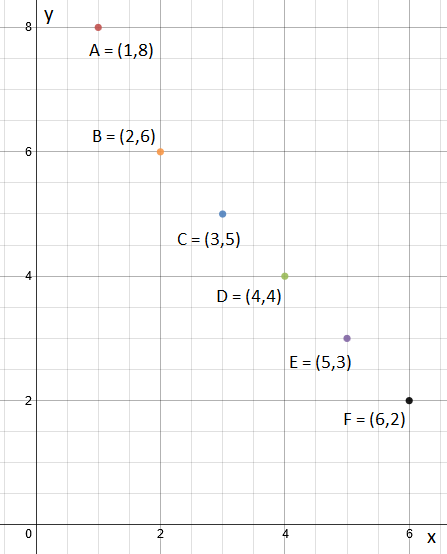
\includegraphics[width=7cm]{EjemploInicialUtil}
  \caption{Puntos distribuidos inicialmente.}
\end{figure}

Primero queremos destruir al objetivo situado en $A$. Miramos el objetivo $B$, que tiene la mayor coordenada $y$ de los que tienen menor coordenada $y$ que $A$ (que son todos dado que se empieza queriendo destruir al objetivo situado en el punto con mayor $y$). En la Figura 2 vemos que $A_{y} > B_{y} + T$ y que A no pertenece al área de impacto A(B, 1), o sea que disparar una genkidama al punto B no eliminaría al androide de A. Por transitividad, como $B_{y} > C_{y} > ... > F_{y}$, ninguno de los disparos a los puntos siguientes a B eliminará al objetivo de A, por lo que es necesario disparar una genkidama a A. El área de impacto A(A, T) = A( (1,8), 1) de esta genkidama, sombrada con rojo en la Figura 2, incluye al punto B, que además es el de mayor coordenada $x$ de los destruidos por esta gendikama.\\
El siguiente a B, C, es el de mayor coordenada $y$ de los que están vivos, y se repite el proceso que se llevó a cabo con A. En la Figura 3 se ve que la segunda gendikama se disparará a D, destruyendo a los objetivos de C, D y E.
Finalmente queda la situación mostrada en la Figura 4 y se dispara una tercera genkidama a F.

\begin{figure}
\centering
\begin{minipage}{.5\textwidth}
  \centering
  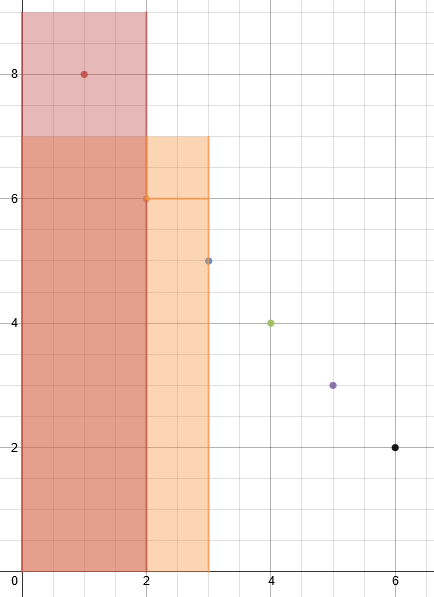
\includegraphics[width=.4\linewidth]{EjemploArea1}
  \caption{Área de impacto de A en rojo y de B en naranja.}
  \label{fig:test1}
\end{minipage}%
\begin{minipage}{.5\textwidth}
  \centering
  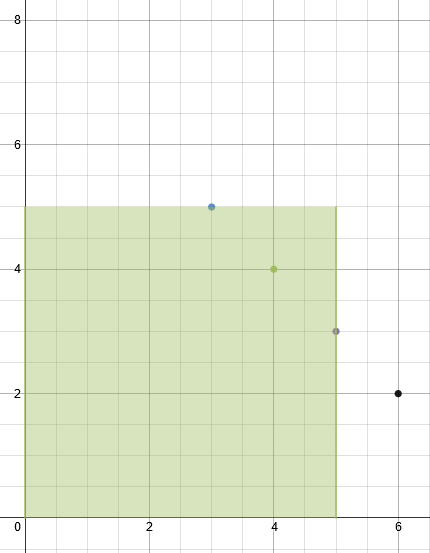
\includegraphics[width=4cm]{EjemploArea2}
  \caption{Área de impacto de D en verde.}
  \label{fig:test2}
\end{minipage}

\begin{minipage}{.5\textwidth}
  \centering
  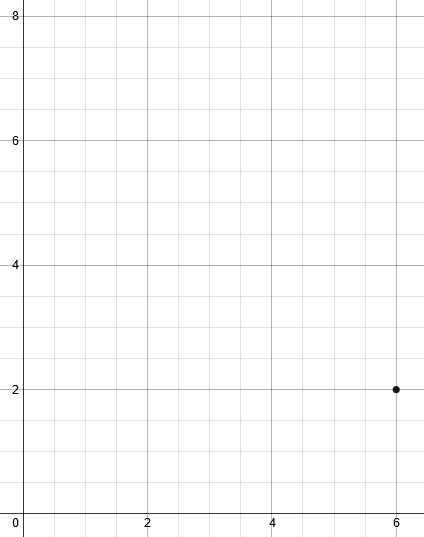
\includegraphics[width=4cm]{EjemploArea3}
  \caption{Androide restante por destruir, en F.}
  \label{fig:test2}
\end{minipage}

\end{figure}

Ahora veamos cómo sería este proceso con $T = 2$.
De vuelta se comienza queriendo destruir al objetivo en A. Como se ve en la Figura 5, disparar a C no destruye a A pero disparar a B sí. Así, morirán los androides situados en los puntos incluidos en la región sombreada naranja en la Figura 6 (el área de impacto A(B, 2)).
Finalmente queda la situación mostrada en la Figura 7 en la que el objetivo es destruir al objetivo de E y se terminará disparando a F eliminando a los dos androides restantes.
En este caso se habrá destruido a todos los androides utilizando dos genkidamas.

\begin{figure}
\centering
\begin{minipage}{.5\textwidth}
  \centering
  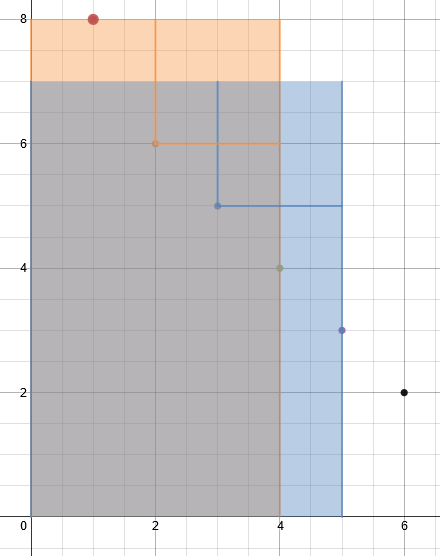
\includegraphics[width=.4\linewidth]{EjemploArea4}
  \caption{Área de impacto de B en naranja y de C en azul.}
  \label{fig:test1}
\end{minipage}%
\begin{minipage}{.5\textwidth}
  \centering
  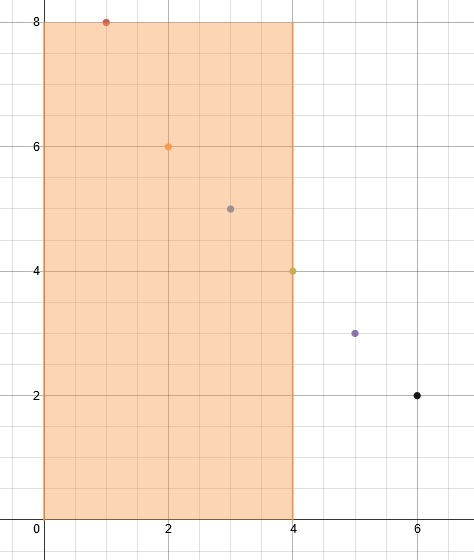
\includegraphics[width=4cm]{EjemploArea5}
  \caption{Área de impacto de B en naranja.}
  \label{fig:test2}
\end{minipage}

\begin{minipage}{.5\textwidth}
  \centering
  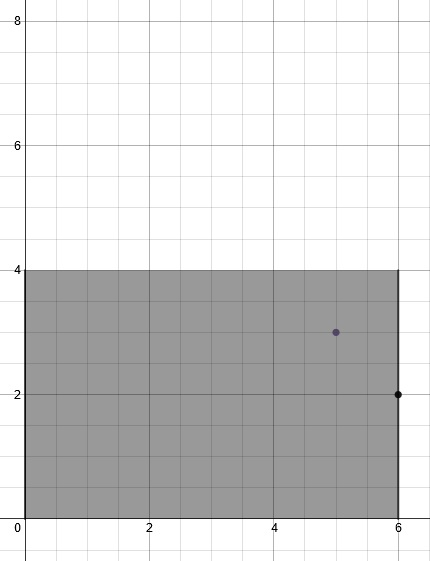
\includegraphics[width=4cm]{EjemploArea6}
  \caption{Área de impacto de F en negro.}
  \label{fig:test2}
\end{minipage}

\end{figure}


\subsection{Ideas para desarrollar el algoritmo}

Definamos el área de impacto como
\begin{gather*}
\textrm{A}:\mathbb{N_{0}}^2 \times \mathbb{N} \rightarrow \mathbb{Z^2}\\
 \mathbf{A}(P,T) = \{ (x, y) \in \mathbb{Z^2} : 0 \leq x \leq P_{x}+T ~ \wedge ~ 0 \leq y \leq P_{y}+T \}
\end{gather*}
 es decir, el conjunto de puntos del plano en los que en caso de haber androides estos morirían por la Gendikama tirada en P. Con esta idea de área de impacto se puede pensar que no aporta tener en cuenta el área por sobre el objetivo vivo de mayor coordenada en y.
Va a haber que eliminar al objetivo situado en A. Se puede tirar una Gendikama al punto A, pero surge la pregunta de si se podría hacer algo mejor. ¿Qué pasa si se dispara a B? Si $ A_{y} \leq B_{y}+T$ entonces el área de impacto A(B,T) incluye al punto A. Así, sería mejor disparar la Gendikama a B que a A dado que como  $A_{x} < B_{x}$ entonces  $A_{x}+T < B_{x}+T$, lo que nos da una idea intuitiva de inclusión de áreas, $A(A,T) \subset A(B,T)$ (nótese que la inclusión es estricta) y podemos decir que diparar a B es más destructivo.
Así, volvemos a preguntarnos: ¿Qué pasa si se dispara a C? ¿Esto también mataría a A?
Si sí, seguimos preguntándonos por el siguiente punto de menor coordenada y, y podemos tener dos situaciones:

\begin{itemize}
\item[•] Recorrer hasta el último punto y que una Gendikama lanzada ahí también elimine al androide situado en A, necesitando sólo un disparo para destruir a todos.
\item[•] Recorrer hasta eventualmente encontrar un androide posicionado en un punto $K$ al que si se lanzara una Gendikama ésta no matara al androide en A. En este caso habría que disparar al androide situado en la posición con la coordenada $y$ inmediatamente anterior a la de $K$, llamémoslo J, y calcular $J_{x}+T$ para ver cuál sería el objetivo de mayor coordenada $y$ que quedara vivo  y repetir el proceso como si este fuera el nuevo $A$. Si no quedara ningún objetivo por eliminar entonces ya no habría necesidad de seguir disparando Gendikamas.
\end{itemize}
\\




\subsection{Pseudocódigo y cota de complejidad}
\begin{algorithm}
\caption{IndiceDeMenorYQueLoMata}
\begin{algorithmic}
  \Function{IndiceDeMenorYQueLoMata}{t: int, indiceDeObjetivo: int, e: $Arreglo<Tupla<int,int>>$}
	\State $int j \gets indiceDeObjetivo - 1$ \Comment $\mathcal{O}(1)$
	\While{$(j \geq 0) && (((e[j]).y + t) \geq (e[indiceDeObjetivo]).y)$} \Comment $\mathcal{indiceDeObjetivo}(1)$
		\State j-~- \Comment $\mathcal{O}(1)$
	\EndWhile
	\State j++ \Comment $\mathcal{O}(1)$
	\State return j \Comment $\mathcal{O}(1)$
\EndFunction
\end{algorithmic}
\underline{Complejidad:} $\mathcal{O}(indiceDeObjetivo)$\\
    
\end{algorithm}


int indiceDeMayorXQueMata(int t, int indiceDeObjetivo, vector<tuple<int,int>> e){
	int distanciaDeDano = get<0>(e[indiceDeObjetivo]) + t;
	int i = indiceDeObjetivo - 1;
	while((i >= 0) && (get<0>(e[i]) <= distanciaDeDano)){
		i--;
	}
	i++;
	return i;
}

void genkidama(int t, int n, vector<tuple<int,int>> e){
	assert (n > 0 && n == e.size() && "La cantidad de enemigos es distinta a la cantidad de posisciones");
	vector<int> atacados;
	int genkidamasUtilizadas = 0;
	int indiceDeObjetivoPorArea = n-1;
	// el de arriba es aquel al que quiero que le llegue la onda expansiva
	bool hayAlgunoVivo = true;
	while(hayAlgunoVivo){
		// el de abajo es aquel al que le voy a tirar la bomba
		int indiceDeObjetivo = indiceDeMenorYQueLoMata(t, indiceDeObjetivoPorArea, e);
		atacados.push_back(indiceDeObjetivo + 1);
		// el +1 de arriba surge de que en el enunciado se enumeran desde el 1 y
		// nosotros enumeramos desde 0
		hayAlgunoVivo = !(indiceDeMayorXQueMata(t, indiceDeObjetivo, e) == 0);
		indiceDeObjetivoPorArea = indiceDeMayorXQueMata(t, indiceDeObjetivo, e) - 1;
		genkidamasUtilizadas++;
		
	}
	std::cout << genkidamasUtilizadas << std::endl;
	int h = 0;
	while (h < genkidamasUtilizadas) {
			std::cout << atacados[h];
			h++;
			if (h < genkidamasUtilizadas) {
					std::cout << " ";
			}
	}
	std::cout << std::endl;
}

\subsection{Experimentacion}
\begin{verbatim}
\end{verbatim}

\newpage
\subsection{Apéndice: código de Genkidama}
\begin{lstlisting}
#include <tuple>
#include <vector>
#include <iostream>
#include <cassert>
using namespace std;

void genkidama(int, int, vector<tuple<int, int>>);
int indiceDeMenorYQueLoMata(int, int, vector<tuple<int,int>>);
int indiceDeMayorXQueMata(int, int, vector<tuple<int,int>>);

int main(){
	int t;
	int n;
	cin >> n >> t;
	vector<tuple<int,int>> e;
	tuple<int,int> en;
	int x;
	int y;
	for (int i = 0; i < n; i++) {
		cin >> x >> y;
		en = make_tuple(x,y);
		e.push_back((en));
	}
	genkidama(t, n, e);
	return 0;
}

// Toma el t, el indice del objetivo en e y el vector de tuplas.
int indiceDeMenorYQueLoMata(int t, int indiceDeObjetivo, vector<tuple<int,int>> e){
	int j = indiceDeObjetivo - 1;
	while((j >= 0) && ((get<1>(e[j]) + t) >= get<1>(e[indiceDeObjetivo]))){
		j--;
	}
	j++;
	return j;
}

int indiceDeMayorXQueMata(int t, int indiceDeObjetivo, vector<tuple<int,int>> e){
	int distanciaDeDano = get<0>(e[indiceDeObjetivo]) + t;
	int i = indiceDeObjetivo - 1;
	while((i >= 0) && (get<0>(e[i]) <= distanciaDeDano)){
		i--;
	}
	i++;
	return i;
}

void genkidama(int t, int n, vector<tuple<int,int>> e){
	assert (n > 0 && n == e.size() && "La cantidad de enemigos es distinta a la cantidad de posisciones");
	vector<int> atacados;
	int genkidamasUtilizadas = 0;
	int indiceDeObjetivoPorArea = n-1;
	// el de arriba es aquel al que quiero que le llegue la onda expansiva
	bool hayAlgunoVivo = true;
	while(hayAlgunoVivo){
		// el de abajo es aquel al que le voy a tirar la bomba
		int indiceDeObjetivo = indiceDeMenorYQueLoMata(t, indiceDeObjetivoPorArea, e);
		atacados.push_back(indiceDeObjetivo + 1);
		// el +1 de arriba surge de que en el enunciado se enumeran desde el 1 y
		// nosotros enumeramos desde 0
		hayAlgunoVivo = !(indiceDeMayorXQueMata(t, indiceDeObjetivo, e) == 0);
		indiceDeObjetivoPorArea = indiceDeMayorXQueMata(t, indiceDeObjetivo, e) - 1;
		genkidamasUtilizadas++;
		
	}
	std::cout << genkidamasUtilizadas << std::endl;
	int h = 0;
	while (h < genkidamasUtilizadas) {
			std::cout << atacados[h];
			h++;
			if (h < genkidamasUtilizadas) {
					std::cout << " ";
			}
	}
	std::cout << std::endl;
}

\end{lstlisting}
\end{document}
